\documentclass[ignorenonframetext]{beamer}
% Note: to generate the actual presentation, comment in the above
% and comment out the following two lines:
%\documentclass{article}
%\usepackage{beamerarticle}

\usepackage{beamerthemesplit}
\usecolortheme{whale}
\usefonttheme[onlymath]{serif}
\usepackage{graphicx}
\usepackage{color}
\usepackage{amsmath}
\usepackage{subfigure}
\useoutertheme{default}

% 1st and second order partial derivative
\newcommand{\pd}[2]{\frac{\partial#1}{\partial#2}}
\newcommand{\pdd}[2]{\frac{\partial^2#1}{\partial#2^2}}
\newcommand{\del}{\triangle}

\begin{document}

\frame{
%\frametitle{Convection-diffusion and Burgers equations}
\begin{figure}
\subfigure[Boundary layer]{
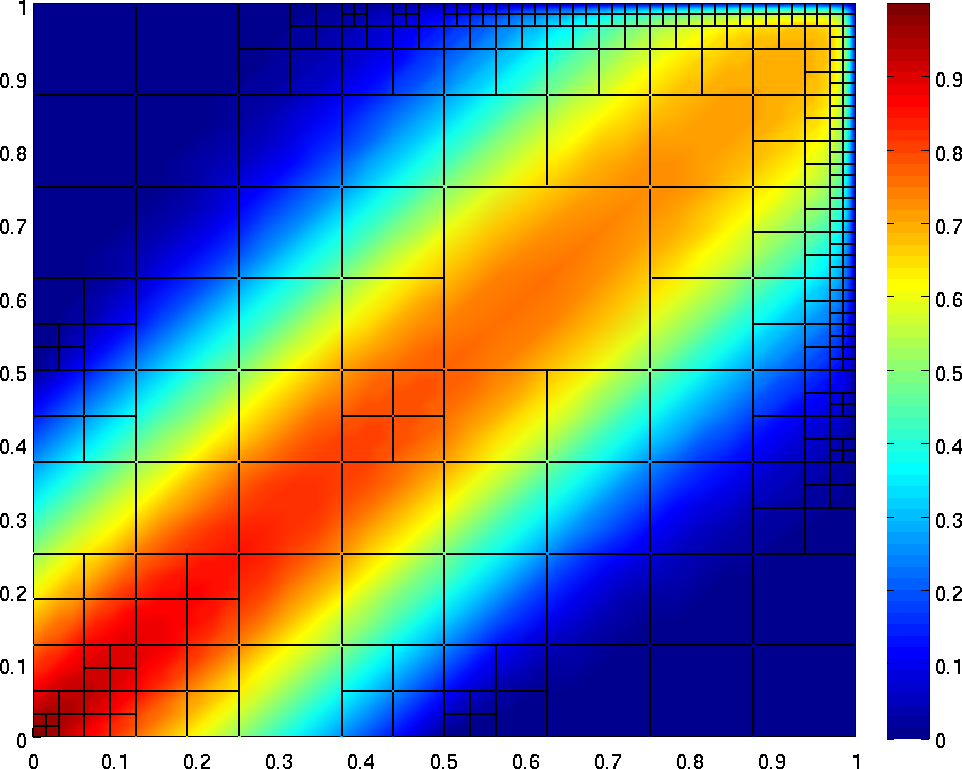
\includegraphics[scale=.23]{confusionDemo.png}
}
\subfigure[Vorticular flow]{
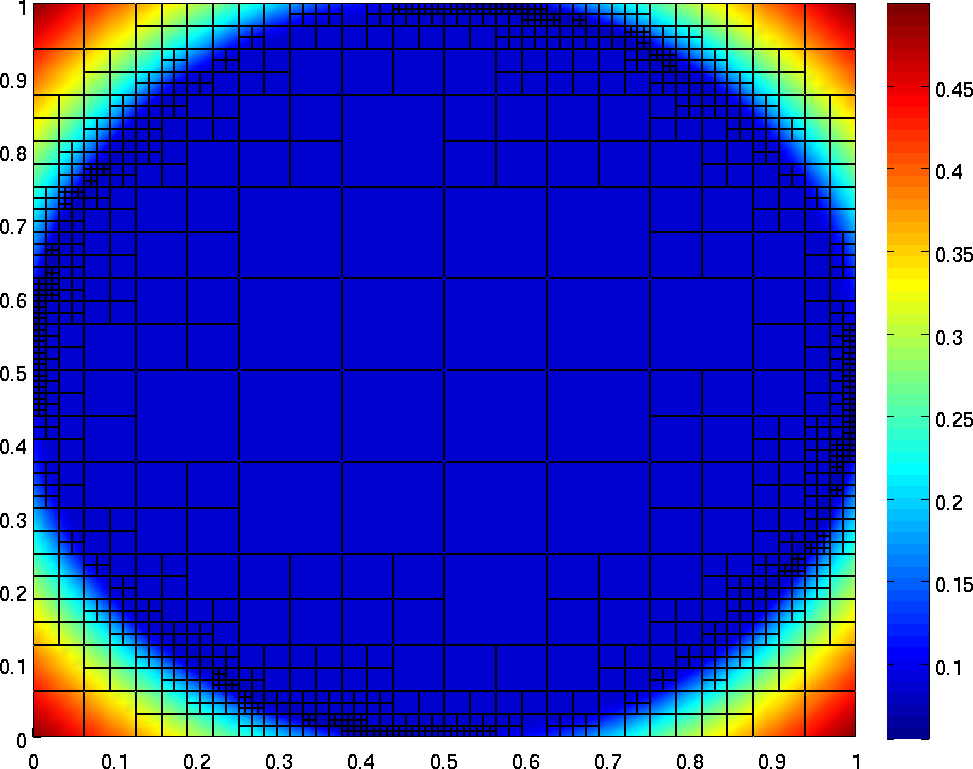
\includegraphics[scale=.23]{confectionDemo.png}
}
\subfigure[Nonlinear shock]{
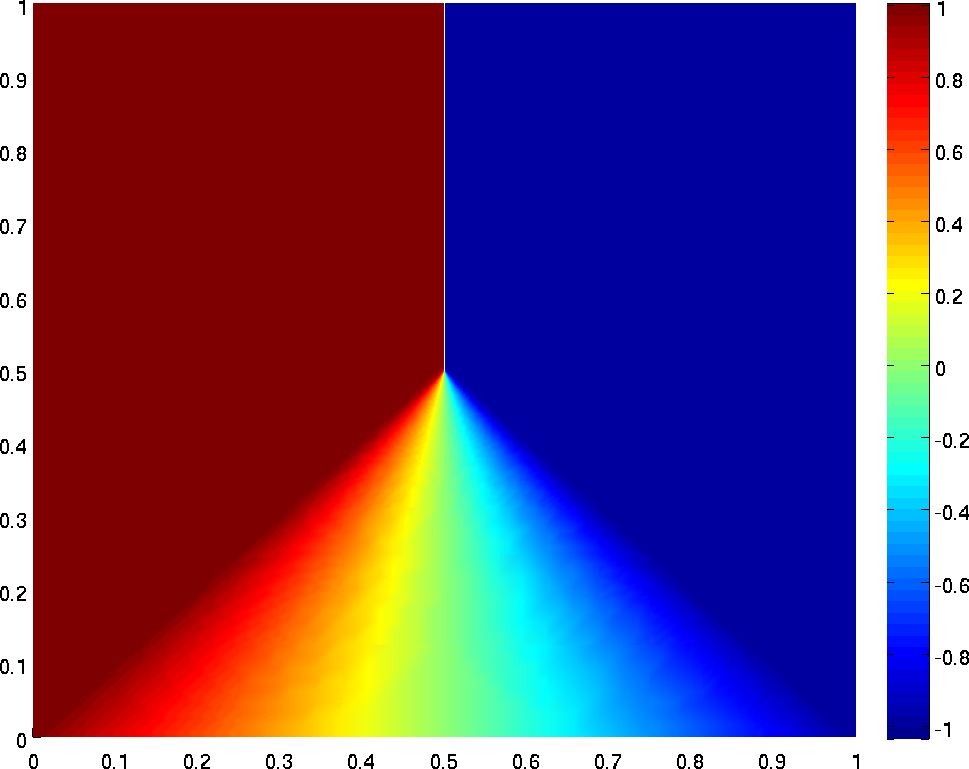
\includegraphics[scale=.23]{burgers1e4.png}
}
\caption{Parallel adaptive solutions using Camellia for convection-diffusion ($\epsilon=1e-2$) and Burgers' equations ($\epsilon=1e-4$).}
\end{figure}
}
\end{document}